\subsection{MyPTV}
\label{sec:locate:myptv}

MyPTV~\cite{myptv} is a Python library developed by Ron Shnapp for 3D particle tracking.
Its \texttt{segmentation} command performs the task of the \locate* step.

\subsubsection{Algorithm}

MyPTV has two different algorithms to perform the \locate* step, ``Labeling'' and ``Dilation''.
The best speed was obtained with ``Labeling'', that is composed by this sequence of steps:
\begin{enumerate}
	\itemsep 0em
	\item Choose all pixels whose gray value is higher than a given threshold;
	\item Pixels that are touching each other are considered to be ``blobs'' and grouped together;
	\item For each blob, the center of mass, the bounding box size and the mass are computed.
\end{enumerate}

\subsubsection{Evaluation}

The output quality is very good, at about 98\% of bubbles correctly identified, as visible in figure~\ref{fig:locate:myptv}.
When concerning the speed, the library achieves 30 FPS, which is better than other approaches, but still only a third of the target speed.

\begin{figure}
	\centerline{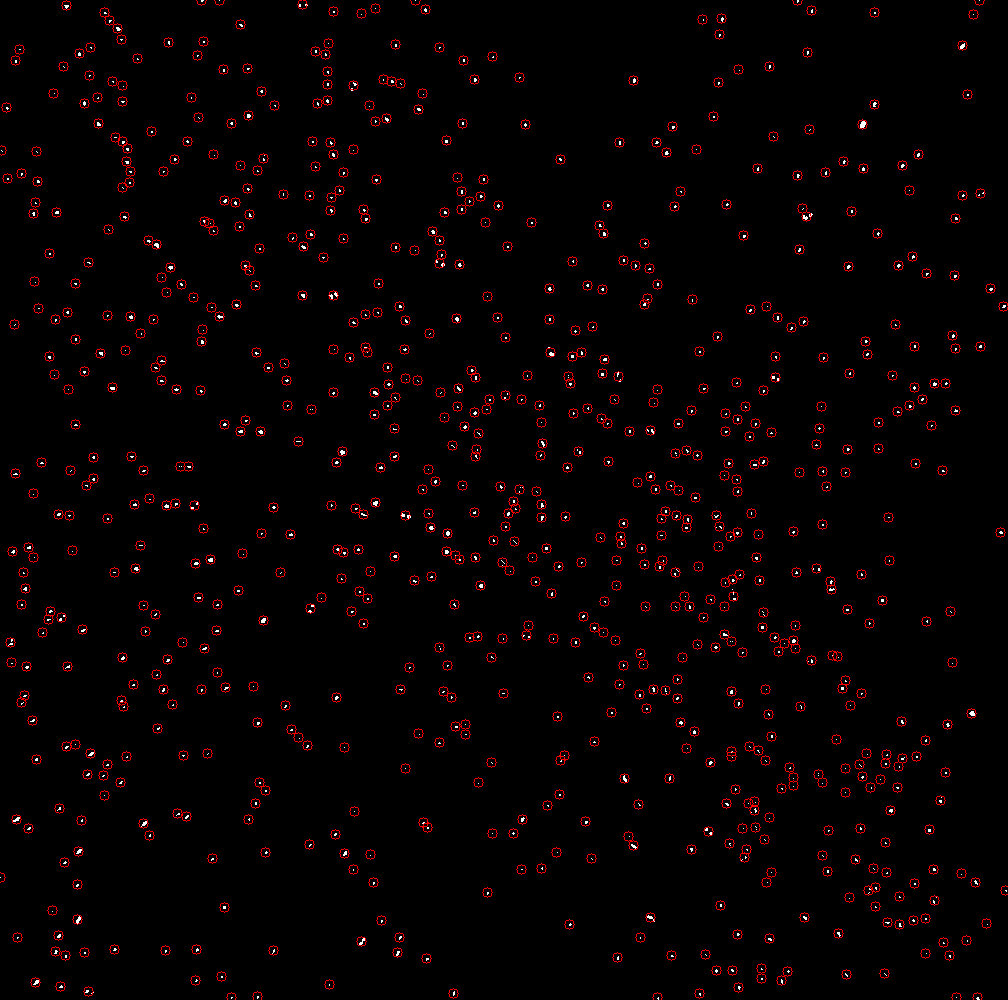
\includegraphics[width=\locateimgsize]{images/locate/myptv.png}}
	\caption{\centering MyPTV's result}
	\label{fig:locate:myptv}
\end{figure}
